\chapter{Модель образования радионуклидов в топливе и теплоносителе ядерного реактора}

\section{Миграция радионуклидов на \ac{aes}}

Как и любое масштабное производство, \ac{aes} выбрасывает в атмосферу и окружающую среду вредные вещества, среди 
которых есть и радиоактивные. При нормальных условиях эксплуатации эти выбросы незначительны, так как современные 
атомные электростанции содержат множество систем очистки сбросов от радионуклидов, однако при нарушении работы 
какой-либо из систем \ac{aes} становится серьезным источником выбросов радионуклидов в атмосферу. 

Хотя принцип работы различных типов ядерных реакторов одинаков, их технологические схемы и устройства различны. В 
данном разделе рассмотрим образование радионуклидов с дальнейшим переходом в теплоноситель первого контура на примере 
реактора типа \ac{vver}.

Основные пути распространения радиоактивных нуклидов на \ac{aes} представлены на рисунке \ref{fig_nuclides_spread}.

\begin{figure}[ht]
\centering
	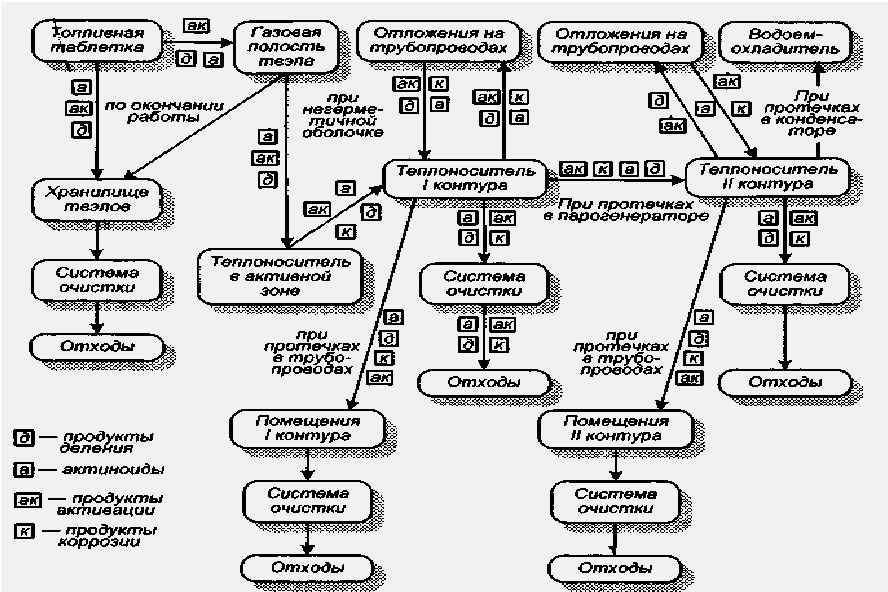
\includegraphics[width=16cm]{nuclides_spread}
    \caption{Основные пути распространения радионуклидов на \ac{aes}.}
    \label{fig_nuclides_spread}
\end{figure}

Топливную таблетку в \ac{tvel}ах рассматривают как первый барьер распространения радиоактивных нуклидов в пределах 
активной зоны ядерного реактора. В результате реакции деления и захвата нейтронов в топливной таблетке накапливаются 
радионуклиды, изменяя состав, физико-химические и механические свойства топливной композиции. При температуре ниже 
1000 \degree C диоксид урана, который наиболее часто используется в качестве топлива в реакторах типа \ac{vver}, 
удерживает практически все радионуклиды, образующиеся в процессе работы реактора. При росте температуры ситуация 
существенно меняется, так как продукты захвата и деления становятся более подвижными \cite{leskin_vver}.

Между топливной таблеткой и оболочкой \ac{tvel}а присутствует небольшой зазор и газовая полость, предназначенные для 
накопления продуктов деления и активации, которым удалось покинуть пределы топливной таблетки.

Вторым барьером распространения радионуклидов является оболочка \ac{tvel}ов. В случае герметичной оболочки \ac{tvel}ов 
выход радионуклидов за пределы оболочки достаточно мал. В реальности, из за высоких тепловых и радиационных нагрузок и 
процессов коррозионно-усталостного типа оболочки теряют свою герметичность. Согласно \cite{kolpakov_tvel}, при 
эксплуатации ядерного реактора пределом безопасной эксплуатации по количеству и величине дефектов составляет 1 \% 
\ac{tvel}ов с дефектами типа газовой неплотности.

В случае разгерметизации топливной оболочки радионуклиды диффундируют через микротрещины в теплоноситель, находящийся 
в активной зоне реактора, который в дальнейшем переходит в первый контур реакторной установки. Более того, 
дополнительным источником радиоактивности в теплоносителе первого контура является его активация нейтронами. 

Часть радионуклидов теплоносителя первого контура при протечках в трубопроводах может попасть в производственные 
помещения первого контура: герметичные боксы и защитную оболочку реактора. При наличии микротрещин или протечек в 
парогенераторе радиоактивность первого контура может перейти в теплоноситель второго контура реакторной установки.
